% Options for packages loaded elsewhere
\PassOptionsToPackage{unicode}{hyperref}
\PassOptionsToPackage{hyphens}{url}
%
\documentclass[
]{article}
\usepackage{amsmath,amssymb}
\usepackage{iftex}
\ifPDFTeX
  \usepackage[T1]{fontenc}
  \usepackage[utf8]{inputenc}
  \usepackage{textcomp} % provide euro and other symbols
\else % if luatex or xetex
  \usepackage{unicode-math} % this also loads fontspec
  \defaultfontfeatures{Scale=MatchLowercase}
  \defaultfontfeatures[\rmfamily]{Ligatures=TeX,Scale=1}
\fi
\usepackage{lmodern}
\ifPDFTeX\else
  % xetex/luatex font selection
\fi
% Use upquote if available, for straight quotes in verbatim environments
\IfFileExists{upquote.sty}{\usepackage{upquote}}{}
\IfFileExists{microtype.sty}{% use microtype if available
  \usepackage[]{microtype}
  \UseMicrotypeSet[protrusion]{basicmath} % disable protrusion for tt fonts
}{}
\makeatletter
\@ifundefined{KOMAClassName}{% if non-KOMA class
  \IfFileExists{parskip.sty}{%
    \usepackage{parskip}
  }{% else
    \setlength{\parindent}{0pt}
    \setlength{\parskip}{6pt plus 2pt minus 1pt}}
}{% if KOMA class
  \KOMAoptions{parskip=half}}
\makeatother
\usepackage{xcolor}
\usepackage[margin=1in]{geometry}
\usepackage{color}
\usepackage{fancyvrb}
\newcommand{\VerbBar}{|}
\newcommand{\VERB}{\Verb[commandchars=\\\{\}]}
\DefineVerbatimEnvironment{Highlighting}{Verbatim}{commandchars=\\\{\}}
% Add ',fontsize=\small' for more characters per line
\usepackage{framed}
\definecolor{shadecolor}{RGB}{248,248,248}
\newenvironment{Shaded}{\begin{snugshade}}{\end{snugshade}}
\newcommand{\AlertTok}[1]{\textcolor[rgb]{0.94,0.16,0.16}{#1}}
\newcommand{\AnnotationTok}[1]{\textcolor[rgb]{0.56,0.35,0.01}{\textbf{\textit{#1}}}}
\newcommand{\AttributeTok}[1]{\textcolor[rgb]{0.13,0.29,0.53}{#1}}
\newcommand{\BaseNTok}[1]{\textcolor[rgb]{0.00,0.00,0.81}{#1}}
\newcommand{\BuiltInTok}[1]{#1}
\newcommand{\CharTok}[1]{\textcolor[rgb]{0.31,0.60,0.02}{#1}}
\newcommand{\CommentTok}[1]{\textcolor[rgb]{0.56,0.35,0.01}{\textit{#1}}}
\newcommand{\CommentVarTok}[1]{\textcolor[rgb]{0.56,0.35,0.01}{\textbf{\textit{#1}}}}
\newcommand{\ConstantTok}[1]{\textcolor[rgb]{0.56,0.35,0.01}{#1}}
\newcommand{\ControlFlowTok}[1]{\textcolor[rgb]{0.13,0.29,0.53}{\textbf{#1}}}
\newcommand{\DataTypeTok}[1]{\textcolor[rgb]{0.13,0.29,0.53}{#1}}
\newcommand{\DecValTok}[1]{\textcolor[rgb]{0.00,0.00,0.81}{#1}}
\newcommand{\DocumentationTok}[1]{\textcolor[rgb]{0.56,0.35,0.01}{\textbf{\textit{#1}}}}
\newcommand{\ErrorTok}[1]{\textcolor[rgb]{0.64,0.00,0.00}{\textbf{#1}}}
\newcommand{\ExtensionTok}[1]{#1}
\newcommand{\FloatTok}[1]{\textcolor[rgb]{0.00,0.00,0.81}{#1}}
\newcommand{\FunctionTok}[1]{\textcolor[rgb]{0.13,0.29,0.53}{\textbf{#1}}}
\newcommand{\ImportTok}[1]{#1}
\newcommand{\InformationTok}[1]{\textcolor[rgb]{0.56,0.35,0.01}{\textbf{\textit{#1}}}}
\newcommand{\KeywordTok}[1]{\textcolor[rgb]{0.13,0.29,0.53}{\textbf{#1}}}
\newcommand{\NormalTok}[1]{#1}
\newcommand{\OperatorTok}[1]{\textcolor[rgb]{0.81,0.36,0.00}{\textbf{#1}}}
\newcommand{\OtherTok}[1]{\textcolor[rgb]{0.56,0.35,0.01}{#1}}
\newcommand{\PreprocessorTok}[1]{\textcolor[rgb]{0.56,0.35,0.01}{\textit{#1}}}
\newcommand{\RegionMarkerTok}[1]{#1}
\newcommand{\SpecialCharTok}[1]{\textcolor[rgb]{0.81,0.36,0.00}{\textbf{#1}}}
\newcommand{\SpecialStringTok}[1]{\textcolor[rgb]{0.31,0.60,0.02}{#1}}
\newcommand{\StringTok}[1]{\textcolor[rgb]{0.31,0.60,0.02}{#1}}
\newcommand{\VariableTok}[1]{\textcolor[rgb]{0.00,0.00,0.00}{#1}}
\newcommand{\VerbatimStringTok}[1]{\textcolor[rgb]{0.31,0.60,0.02}{#1}}
\newcommand{\WarningTok}[1]{\textcolor[rgb]{0.56,0.35,0.01}{\textbf{\textit{#1}}}}
\usepackage{longtable,booktabs,array}
\usepackage{calc} % for calculating minipage widths
% Correct order of tables after \paragraph or \subparagraph
\usepackage{etoolbox}
\makeatletter
\patchcmd\longtable{\par}{\if@noskipsec\mbox{}\fi\par}{}{}
\makeatother
% Allow footnotes in longtable head/foot
\IfFileExists{footnotehyper.sty}{\usepackage{footnotehyper}}{\usepackage{footnote}}
\makesavenoteenv{longtable}
\usepackage{graphicx}
\makeatletter
\def\maxwidth{\ifdim\Gin@nat@width>\linewidth\linewidth\else\Gin@nat@width\fi}
\def\maxheight{\ifdim\Gin@nat@height>\textheight\textheight\else\Gin@nat@height\fi}
\makeatother
% Scale images if necessary, so that they will not overflow the page
% margins by default, and it is still possible to overwrite the defaults
% using explicit options in \includegraphics[width, height, ...]{}
\setkeys{Gin}{width=\maxwidth,height=\maxheight,keepaspectratio}
% Set default figure placement to htbp
\makeatletter
\def\fps@figure{htbp}
\makeatother
\usepackage{soul}
\setlength{\emergencystretch}{3em} % prevent overfull lines
\providecommand{\tightlist}{%
  \setlength{\itemsep}{0pt}\setlength{\parskip}{0pt}}
\setcounter{secnumdepth}{-\maxdimen} % remove section numbering
\ifLuaTeX
  \usepackage{selnolig}  % disable illegal ligatures
\fi
\IfFileExists{bookmark.sty}{\usepackage{bookmark}}{\usepackage{hyperref}}
\IfFileExists{xurl.sty}{\usepackage{xurl}}{} % add URL line breaks if available
\urlstyle{same}
\hypersetup{
  pdftitle={Multiple Imputation in R},
  pdfauthor={Maria Sanchez and Marta Pineda-Moncusi},
  hidelinks,
  pdfcreator={LaTeX via pandoc}}

\title{Multiple Imputation in R}
\author{Maria Sanchez and Marta Pineda-Moncusi}
\date{2023-11-12}

\begin{document}
\maketitle

/* Whole document: */ body\{ font-family: Helvetica; font-size: 16pt; \}

\begin{Shaded}
\begin{Highlighting}[]
\FunctionTok{rm}\NormalTok{(}\AttributeTok{list=}\FunctionTok{ls}\NormalTok{())}
\end{Highlighting}
\end{Shaded}

\hypertarget{tutorial-for-multiple-imputation-in-r}{%
\section{Tutorial for Multiple Imputation in
R}\label{tutorial-for-multiple-imputation-in-r}}

\hypertarget{introduction}{%
\subsection{Introduction}\label{introduction}}

Missing data (or missing values) is defined as the data value that is
not stored for a variable in the observation of interest. The problem of
missing data is relatively common in almost all research and can have a
significant effect on the conclusions that can be drawn from the data.

A common misconception of missing data methods is the assumption that
imputed values should represent ``real'' values. The purpose when
addressing missing data is to correctly reproduce the
variance/covariance matrix we would have observed if our data had not
any missing information.

The aim of this practical is to discuss commonly used techniques for
handling missing data and common issues that could arise when these
techniques are used. We will focus on one of the most popular methods,
\textbf{multiple imputation}. But, depending on the type of data and
model you will be using, other techniques such as direct maximum
likelihood may better serve your needs.

We will use the data set \textbf{\emph{hip.csv}}. This data set is made
up for this practical. The R code for this practical was developed using
R 4.2.1 version.

\hypertarget{load-and-evaluate-the-data-set}{%
\subsection{Load and evaluate the data
set}\label{load-and-evaluate-the-data-set}}

\textbf{The Hip Replacement (HIP) data set}

The hip data set contains information on seven hundred and eight
patients receiving primary hip replacement surgery for osteoarthritis
(variable \texttt{id} is the unique patient identifier). Prior to the
operation, patients completed a pre-operative Oxford Hip Score (OHS) and
EQ5D (Euroqol) questionnaire with a follow-up questionnaire being filled
in at 6-months post-surgery. The OHS consists of 12 questions asking
patients to describe their hip pain and function during the past 4
weeks. An overall score is created by summing the responses to each of
the 12 questions, ranging from 0 to 48, where 0 is the worst possible
score (severe symptoms) and 48 the best score (excellent joint
function). Variable \texttt{ohs0} is the preoperative score and
\texttt{ohs6} post-operative. The absolute change in OHS between pre-
and post-operative assessments (variable \texttt{ohsdiff}) is negative
if patient symptoms have improved and positive for worsening.

The pre-operative \texttt{eq5d0} contains information from 5 questions
asking about a patient's health state today, covering mobility,
self-care, usual activities, pain, and anxiety. The \texttt{eq5d0} has
been converted to a single summary score (variable \texttt{eq5d0}),
anchored at 0 for death and 1 for full health, with some health states
being worse than dead (-0.594).

Six months after their operation patients were asked about their overall
satisfaction with the outcome of surgery measured on a visual analogue
scale from 0 to 100 (variable \texttt{satisfaction}).

Pre-operative information was collected on \texttt{age} at the time of
surgery, \texttt{sex} (0 = Male; 1 = Female), \texttt{height} (metres)
and \texttt{weight} (kg) (from which body mass index (\texttt{bmi}) is
calculated), \texttt{side} of surgery (Left; Right), \texttt{ethnic}
group (0 = White; 1 = Non white), whether or not they are
\texttt{retired} (0 = Not retired; 1 = Retired), \texttt{smoking} (0 =
Non-smoker; 1 = Smoker) and \texttt{occupation} is defined as 1 if the
individual is a manual worked and 0 if not. The Index of Multiple
Deprivation is a measure of social deprivation, linked to the area a
patient lives in (variable \texttt{imdscore})

\begin{Shaded}
\begin{Highlighting}[]
\CommentTok{\#install.packages("dplyr")}
\FunctionTok{library}\NormalTok{(dplyr)}
\FunctionTok{library}\NormalTok{(tibble)}

\CommentTok{\#See your working directory}
\FunctionTok{getwd}\NormalTok{()}

\CommentTok{\#Update your working directory to the folder where "hip.data" is stored (if necessary)}
\NormalTok{update\_wd }\OtherTok{=} \StringTok{"NO"} \CommentTok{\#"NO" for keeping the current working directory. "YES" to update, plus including the new path in folder\_path variable below.}
\ControlFlowTok{if}\NormalTok{(update\_wd }\SpecialCharTok{==} \StringTok{"YES"}\NormalTok{)\{}
\NormalTok{folder\_path }\OtherTok{\textless{}{-}}\NormalTok{ (}\StringTok{"C:/"}\NormalTok{)  }\CommentTok{\#Remind to use / (NOT \textbackslash{})}
\FunctionTok{setwd}\NormalTok{(folder\_path)}
\NormalTok{\}}

\CommentTok{\#load data}
\NormalTok{data }\OtherTok{\textless{}{-}} \FunctionTok{tibble}\NormalTok{(}\FunctionTok{read.csv}\NormalTok{(}\StringTok{"hip.csv"}\NormalTok{, }\AttributeTok{sep=}\StringTok{\textquotesingle{},\textquotesingle{}}\NormalTok{))}


\CommentTok{\#Display the names of variables in the data set.}
\FunctionTok{names}\NormalTok{(data)}

\CommentTok{\#transform/include labels to data}
\NormalTok{data }\OtherTok{=}\NormalTok{ data }\SpecialCharTok{\%\textgreater{}\%} 
            \FunctionTok{mutate}\NormalTok{(}\AttributeTok{sex =} \FunctionTok{factor}\NormalTok{(sex, }\AttributeTok{levels =} \FunctionTok{c}\NormalTok{(}\DecValTok{0}\NormalTok{,}\DecValTok{1}\NormalTok{), }\AttributeTok{labels =} \FunctionTok{c}\NormalTok{(}\StringTok{"Male"}\NormalTok{,}\StringTok{"Female"}\NormalTok{)),}
                 \AttributeTok{retired =} \FunctionTok{factor}\NormalTok{(retired, }\AttributeTok{levels =} \FunctionTok{c}\NormalTok{(}\DecValTok{0}\NormalTok{,}\DecValTok{1}\NormalTok{), }\AttributeTok{labels =} \FunctionTok{c}\NormalTok{(}\StringTok{"Not retired"}\NormalTok{,}\StringTok{"Retired"}\NormalTok{)),}
                 \AttributeTok{ethnic =} \FunctionTok{factor}\NormalTok{(ethnic, }\AttributeTok{levels =} \FunctionTok{c}\NormalTok{(}\DecValTok{0}\NormalTok{,}\DecValTok{1}\NormalTok{), }\AttributeTok{labels =} \FunctionTok{c}\NormalTok{(}\StringTok{"White"}\NormalTok{,}\StringTok{"Non white"}\NormalTok{)),}
                 \AttributeTok{side =} \FunctionTok{factor}\NormalTok{(side, }\AttributeTok{levels =} \FunctionTok{c}\NormalTok{(}\DecValTok{0}\NormalTok{,}\DecValTok{1}\NormalTok{), }\AttributeTok{labels =} \FunctionTok{c}\NormalTok{(}\StringTok{"Right"}\NormalTok{,}\StringTok{"Left"}\NormalTok{)),}
                 \AttributeTok{smoking =} \FunctionTok{factor}\NormalTok{(smoking, }\AttributeTok{levels =} \FunctionTok{c}\NormalTok{(}\DecValTok{0}\NormalTok{,}\DecValTok{1}\NormalTok{), }\AttributeTok{labels =} \FunctionTok{c}\NormalTok{(}\StringTok{"Non{-}smoker"}\NormalTok{,}\StringTok{"Smoker"}\NormalTok{)),}
                 \AttributeTok{occupation =} \FunctionTok{factor}\NormalTok{(data}\SpecialCharTok{$}\NormalTok{occupation, }\AttributeTok{levels =} \FunctionTok{c}\NormalTok{(}\DecValTok{0}\NormalTok{,}\DecValTok{1}\NormalTok{), }\AttributeTok{labels =} \FunctionTok{c}\NormalTok{(}\StringTok{"Non{-}manual worker"}\NormalTok{,}\StringTok{"Manual worker"}\NormalTok{)) )}

\CommentTok{\#Observe/explore the data}
\FunctionTok{dim}\NormalTok{(data)}
\FunctionTok{summary}\NormalTok{(data)}
\end{Highlighting}
\end{Shaded}

\textbf{Quiz}

\ul{\emph{Check the structure of the data}}:

\begin{itemize}
\item
  How many cases (individuals) are in the data?
\item
  How many variables do we have?
\item
  Which are numeric?
\item
  Which are factor?
\item
  Is there any variable with missing values?
\item
  Describe the outcome:

  \begin{center}\rule{0.5\linewidth}{0.5pt}\end{center}
\end{itemize}

\hypertarget{exploring-missing-data-mechanisms}{%
\subsection{Exploring missing data
mechanisms}\label{exploring-missing-data-mechanisms}}

There are three typical mechanisms causing missing data:

\begin{itemize}
\tightlist
\item
  Missing completely at random (MCAR): The probability of data being
  missing is the same for all cases (not dependent on the observed or
  unobserved data)

  \begin{itemize}
  \tightlist
  \item
    In the presence of MCAR, complete cases analysis will not depend
    results in biased parameter estimates (e.g.~regression coefficients)
  \end{itemize}
\item
  Missing at random (MAR): The probability of data being missing is the
  same only within groups defined by the observed data.

  \begin{itemize}
  \tightlist
  \item
    In the presence of MAR, \textbf{multiple imputation} methods may
    lead to unbiased results
  \end{itemize}
\item
  Missing not at random (MNAR): The probability of data being missing
  varies for reasons that are unknown to us or does depend on the
  unobserved data, conditional on the observed data
\end{itemize}

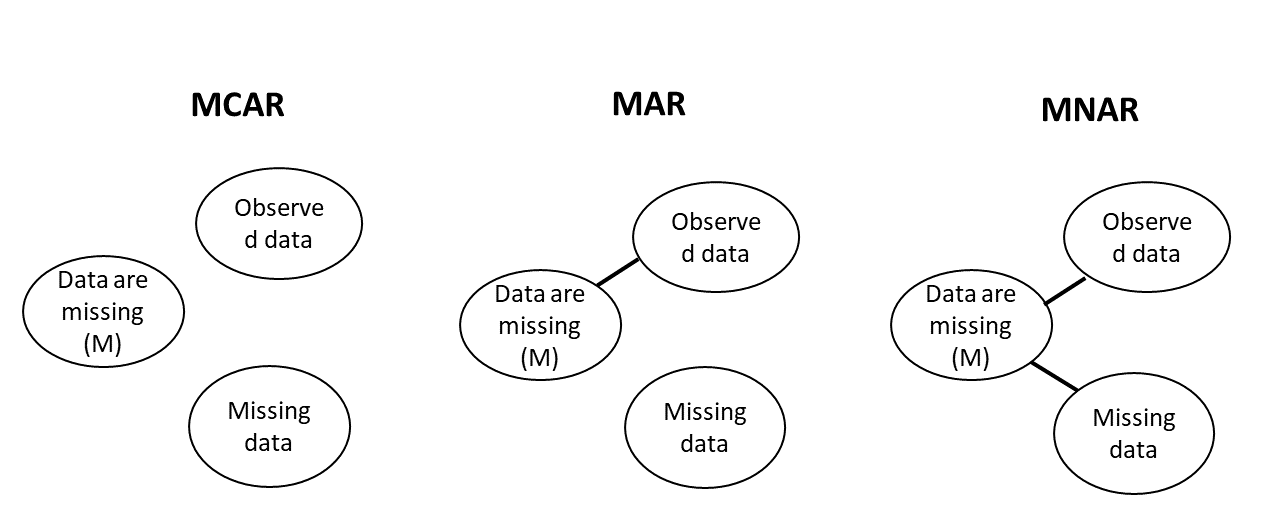
\includegraphics{images/Types of missing data.png}

To explore the mechanism of the missing data in our data set, we can
check if missingness are associated with completed variables.

\begin{enumerate}
\def\labelenumi{\arabic{enumi}.}
\tightlist
\item
  We can check if missing values are associated to observed variables
  using a correlation matrix:
\end{enumerate}

\begin{Shaded}
\begin{Highlighting}[]
\CommentTok{\#list the variables you want to test}
\NormalTok{miss\_var\_list }\OtherTok{=} \FunctionTok{c}\NormalTok{(}\StringTok{"eq5d0"}\NormalTok{, }\StringTok{"ethnic"}\NormalTok{, }\StringTok{"imdscore"}\NormalTok{, }\StringTok{"bmi"}\NormalTok{, }\StringTok{"smoking"}\NormalTok{)}
\NormalTok{complete\_var  }\OtherTok{=} \FunctionTok{c}\NormalTok{(}\StringTok{"age"}\NormalTok{, }\StringTok{"sex"}\NormalTok{, }\StringTok{"ohsdiff"}\NormalTok{,}\StringTok{"ohs0"}\NormalTok{)}

\CommentTok{\#install.packages("ggcorrplot")}
\FunctionTok{library}\NormalTok{(ggcorrplot)}

\CommentTok{\#Generate a data frame where missing variables are codified by 0=non{-}missing value and 1=missing value:}
\NormalTok{miss\_data }\OtherTok{=}\NormalTok{  data }\SpecialCharTok{\%\textgreater{}\%} \FunctionTok{mutate}\NormalTok{(}
  \AttributeTok{miss\_eq5d0=} \FunctionTok{ifelse}\NormalTok{(}\FunctionTok{is.na}\NormalTok{(eq5d0),}\DecValTok{1}\NormalTok{,}\DecValTok{0}\NormalTok{), }
  \AttributeTok{miss\_ethnic=} \FunctionTok{ifelse}\NormalTok{(}\FunctionTok{is.na}\NormalTok{(ethnic),}\DecValTok{1}\NormalTok{,}\DecValTok{0}\NormalTok{), }
  \AttributeTok{miss\_imdscore=} \FunctionTok{ifelse}\NormalTok{(}\FunctionTok{is.na}\NormalTok{(imdscore),}\DecValTok{1}\NormalTok{,}\DecValTok{0}\NormalTok{), }
  \AttributeTok{miss\_bmi=}\FunctionTok{ifelse}\NormalTok{(}\FunctionTok{is.na}\NormalTok{(bmi),}\DecValTok{1}\NormalTok{,}\DecValTok{0}\NormalTok{), }
  \AttributeTok{miss\_smoking=} \FunctionTok{ifelse}\NormalTok{(}\FunctionTok{is.na}\NormalTok{(smoking),}\DecValTok{1}\NormalTok{,}\DecValTok{0}\NormalTok{) )}

\NormalTok{corr\_var }\OtherTok{=} \FunctionTok{c}\NormalTok{(}\StringTok{"miss\_eq5d0"}\NormalTok{, }\StringTok{"miss\_ethnic"}\NormalTok{, }\StringTok{"miss\_imdscore"}\NormalTok{, }\StringTok{"miss\_bmi"}\NormalTok{, }\StringTok{"miss\_smoking"}\NormalTok{, complete\_var)}

\FunctionTok{model.matrix}\NormalTok{(}\SpecialCharTok{\textasciitilde{}}\DecValTok{0}\SpecialCharTok{+}\NormalTok{., }\AttributeTok{data=}\NormalTok{miss\_data[corr\_var]) }\SpecialCharTok{\%\textgreater{}\%} 
  \FunctionTok{cor}\NormalTok{(}\AttributeTok{use=}\StringTok{"pairwise.complete.obs"}\NormalTok{)  }\SpecialCharTok{\%\textgreater{}\%} 
  \FunctionTok{ggcorrplot}\NormalTok{(}\AttributeTok{show.diag =}\NormalTok{ F, }\AttributeTok{type=}\StringTok{"lower"}\NormalTok{, }\AttributeTok{lab=}\ConstantTok{TRUE}\NormalTok{, }\AttributeTok{lab\_size=}\DecValTok{2}\NormalTok{)}
\end{Highlighting}
\end{Shaded}

\begin{itemize}
\tightlist
\item
  What is the correlation between bmi and ethnic missingnes? how does it
  mean? The correlation is 0.99, and that means that the variables bmi
  and ethnic have almost the same missing values.
\end{itemize}

\begin{enumerate}
\def\labelenumi{\arabic{enumi}.}
\setcounter{enumi}{1}
\tightlist
\item
  Create a dummy variable/s where missing values are classified as 1 and
  complete values as 0, then we run a logistic regression:
\end{enumerate}

\begin{Shaded}
\begin{Highlighting}[]
\CommentTok{\#list the variables you want to test}
\NormalTok{miss\_var\_list }\OtherTok{=} \FunctionTok{c}\NormalTok{(}\StringTok{"eq5d0"}\NormalTok{, }\StringTok{"bmi"}\NormalTok{, }\StringTok{"ethnic"}\NormalTok{, }\StringTok{"imdscore"}\NormalTok{,}\StringTok{"smoking"}\NormalTok{)}
\NormalTok{complete\_var  }\OtherTok{=} \FunctionTok{c}\NormalTok{(}\StringTok{"age"}\NormalTok{, }\StringTok{"sex"}\NormalTok{, }\StringTok{"retired"}\NormalTok{, }\StringTok{"ohsdiff"}\NormalTok{,}\StringTok{"side"}\NormalTok{,}\StringTok{"occupation"}\NormalTok{)}

\ControlFlowTok{for}\NormalTok{ (v }\ControlFlowTok{in} \DecValTok{1}\SpecialCharTok{:}\FunctionTok{length}\NormalTok{(miss\_var\_list))\{}
\NormalTok{ miss\_var }\OtherTok{=} \FunctionTok{ifelse}\NormalTok{(}\FunctionTok{is.na}\NormalTok{(data[[miss\_var\_list[v]]]), }\DecValTok{1}\NormalTok{, }\DecValTok{0}\NormalTok{)}
\NormalTok{ test }\OtherTok{=} \FunctionTok{glm}\NormalTok{(miss\_var }\SpecialCharTok{\textasciitilde{}}\NormalTok{ ., }\AttributeTok{data=}\NormalTok{data[complete\_var] )}
 \FunctionTok{print}\NormalTok{(}\FunctionTok{paste}\NormalTok{(}\StringTok{"Tested variable: "}\NormalTok{, miss\_var\_list[v], }\AttributeTok{sep=}\StringTok{""}\NormalTok{)) }
 \FunctionTok{print}\NormalTok{(}\FunctionTok{summary}\NormalTok{(test))   }\CommentTok{\#Check p\_value}
\NormalTok{\}}
\end{Highlighting}
\end{Shaded}

\begin{enumerate}
\def\labelenumi{\arabic{enumi}.}
\setcounter{enumi}{2}
\tightlist
\item
  Alternative, we can use the function na.test() from the package misty:
  This function tests all your data set.
\end{enumerate}

\begin{Shaded}
\begin{Highlighting}[]
\CommentTok{\#install.packages("misty")}
\FunctionTok{library}\NormalTok{(misty)}

\CommentTok{\#We are excluding \textquotesingle{}id\textquotesingle{} from the dataset.}
\FunctionTok{na.test}\NormalTok{(}\FunctionTok{within}\NormalTok{(data, }\FunctionTok{rm}\NormalTok{(id)))}
\end{Highlighting}
\end{Shaded}

\ul{\emph{Interpretation of the function na.test()}}\emph{:}

If the output is statistically significant p-value (p≤0.05), indicates
that the result provides evidence against ``Missing Completely at
Random'' (MCAR) and therefore, the missing data are MAR or MNAR. In this
situation, complete cases analysis will give bias results, therefore,
you need to impute.

If the result is not statistically significant p\textgreater0.05,
indicates that the test is failing to reject the null hypothesis. But,
it doesn't prove that the data is MCAR, so data might or not be MCAR. If
you suspect that an unobserved variable/s may explain the missingness of
your data, you still need to impute your data, assuming that it is MAR.

\begin{center}\rule{0.5\linewidth}{0.5pt}\end{center}

\hypertarget{multiple-imputation-in-r}{%
\subsection{Multiple Imputation in R}\label{multiple-imputation-in-r}}

Multiple imputation is a simulation-based statistical technique for
handling missing data. It is now accepted as the best general method to
deal with incomplete data. Multiple imputation was developed by Donal B.
Rubin in the 1970's.

\hypertarget{procedure}{%
\subsubsection{1. Procedure}\label{procedure}}

Multiple imputation creates more than one complete data sets (m). Each
of these data sets is analysed by standard analysis software. The m
results are pooled into a final point estimate plus standard error by
pooling rules (``Ruben's rules'').

Multiple imputation consists of three steps: imputation, analysis and
pooling.

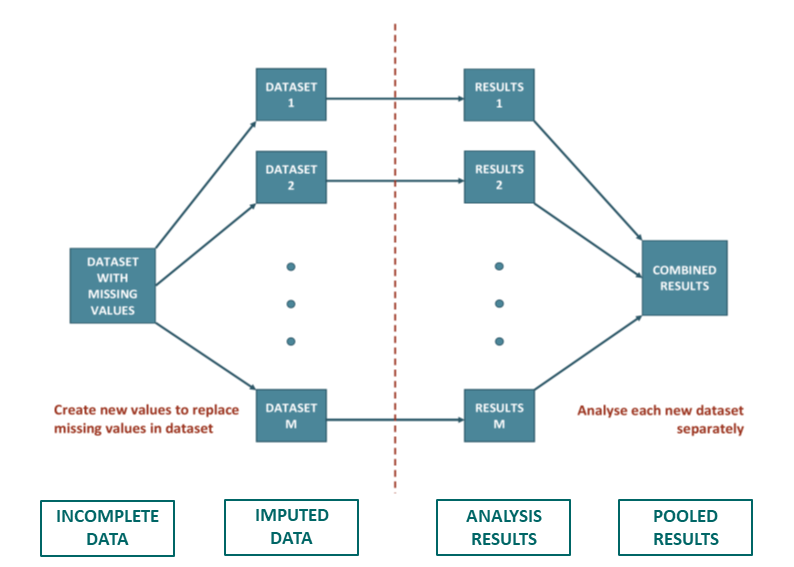
\includegraphics{images/Multiple imputation steps.png}

\begin{itemize}
\item
  \emph{Imputed data:} it creates several complete data (m) sets where
  missing values are replaced by plausible data values. Plausible values
  are taken from the distribution modeled for each missing entry.
\item
  \emph{Analysis results:} it estimates the parameters of interest from
  each imputed data set.
\item
  \emph{Pooled results:} it pools the m parameter estimates into one
  estimate, and to estimate the variance. The variance combines the
  ``within-imputation variance'' and the ``between-imputation
  variance''.

  \begin{center}\rule{0.5\linewidth}{0.5pt}\end{center}
\end{itemize}

\hypertarget{preparing-to-conduct-multiple-imputation}{%
\subsubsection{2. Preparing to conduct Multiple
Imputation}\label{preparing-to-conduct-multiple-imputation}}

\begin{quote}
\textbf{NOTE:} The standard implementation of multiple imputation is
based on the assumption of data being at least MAR.
\end{quote}

When developing your imputation model, it is important to assess if your
imputation model is consistent with your analytic model. Consistency
means that your imputation model includes (at the very least) the same
variables that are in your analytic or estimation model. This also
includes any transformations to variables (e.g.~log transformations,
interactions) that will be needed to assess your hypothesis of interest.

For example, if the analytic model has significant interactions, then
the imputation model should include them as well, if the analytic model
uses a transformed version of a variable then the imputation model
should use the same transformation.

Our analytic model contains:

\begin{itemize}
\tightlist
\item
  The outcome/dependent variable (\emph{Y}) is \texttt{ohsdiff} = change
  in ohs before and after surgery
\item
  The independent variables (\emph{X's}) are = \texttt{age},
  \texttt{sex}, \texttt{ethnic}, \texttt{imdscore} , \texttt{bmi},
  \texttt{smoking} , \texttt{eq5d0} and \texttt{ohs0}
\end{itemize}

We are going to follow the next steps to built the imputation model:

\hypertarget{examine-the-number-of-missing-values-among-your-variables-of-interest}{%
\paragraph{2.1. Examine the number of missing values among your
variables of
interest}\label{examine-the-number-of-missing-values-among-your-variables-of-interest}}

We use the command \texttt{summary} command to count the number of
missing observations of missing for each variable of interest

\begin{Shaded}
\begin{Highlighting}[]
\CommentTok{\#Selecting variables of interest}
\NormalTok{analytic\_model }\OtherTok{\textless{}{-}} \FunctionTok{c}\NormalTok{(}\StringTok{"ohsdiff"}\NormalTok{,}\StringTok{"age"}\NormalTok{, }\StringTok{"sex"}\NormalTok{, }\StringTok{"ethnic"}\NormalTok{, }\StringTok{"eq5d0"}\NormalTok{, }\StringTok{"imdscore"}\NormalTok{, }\StringTok{"bmi"}\NormalTok{, }\StringTok{"smoking"}\NormalTok{, }\StringTok{"ohs0"}\NormalTok{)}

\CommentTok{\#Observe/explore number of missing data}
\FunctionTok{summary}\NormalTok{(data[analytic\_model])}
\end{Highlighting}
\end{Shaded}

\textbf{Quiz}

\begin{itemize}
\tightlist
\item
  Which is the variable with higher number of missing data?
\end{itemize}

\textbf{NOTE}: At this point, you can decide if you want to remove
variables with a high number of missingness from the analytic model, and
therefore, for the imputation model, as they might mess up the
imputation.

\hypertarget{missing-value-patterns}{%
\paragraph{2.2. Missing value patterns}\label{missing-value-patterns}}

Types of missing data
patterns:\href{https://stefvanbuuren.name/fimd/about-the-author.html}{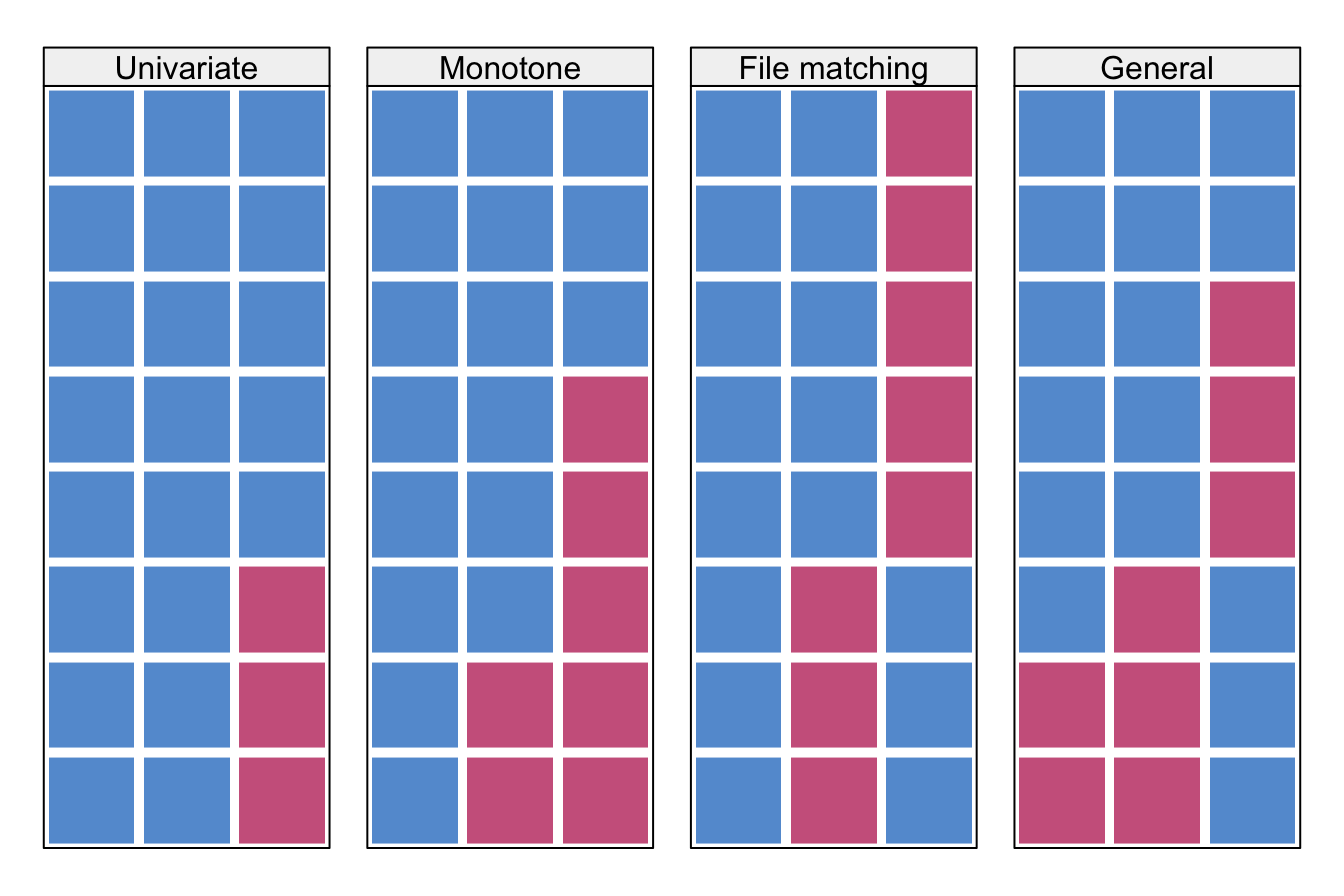
\includegraphics[width=6.54167in,height=\textheight]{images/missing value patterns.png}}\\
\emph{Source: Flexible Imputation of Missing Data, Second Edition.
Author: Stefvan Buuren}

Some missing data patterns in multivariate data. Blue is observed, red
is missing:

\begin{enumerate}
\def\labelenumi{\arabic{enumi}.}
\tightlist
\item
  \emph{Univariate and multivariate}. A missing data pattern is said to
  be \emph{univariate} if there is only one variable with missing data.
\item
  \emph{Monotone and non-monotone (or general)}. A missing data pattern
  is said to be \emph{monotone} when, if the variables are ordered from
  least to most missing, then all observations of a variable contain
  missing in the observations in which the prior variable contains
  missing (\emph{it can occur as a result of drop-out in longitudinal
  studies}). If the pattern is not monotone, it is called
  \emph{non-monotone or general}
\item
  \emph{Unconnected and connected (file matching)}. A missing data
  pattern is said to be \emph{connected} if any observed data point can
  be reached from any other observed data point through a sequence of
  horizontal or vertical moves (like the rook in chess).
\end{enumerate}

The missing data pattern influences the amount of information that can
be transferred between variables.

Imputation can be more precise if other variables are non-missing for
those cases that are to be imputed. The reverse is also true. Predictors
are potentially more powerful if they have are non-missing in rows that
are vastly incomplete. This section discusses various measures of the
missing data pattern.

R has several functions to inspect the missing data pattern.

The mice package contains a function to inspect the missing data
pattern: \texttt{md.pattern()}

\begin{Shaded}
\begin{Highlighting}[]
\CommentTok{\#Selecting variables with missing data}
\NormalTok{miss\_vars }\OtherTok{\textless{}{-}} \FunctionTok{c}\NormalTok{( }\StringTok{"eq5d0"}\NormalTok{, }\StringTok{"ethnic"}\NormalTok{,}\StringTok{"imdscore"}\NormalTok{, }\StringTok{"bmi"}\NormalTok{, }\StringTok{"smoking"}\NormalTok{)}

\CommentTok{\#Exploring missing pattern with md.pattern() function}
\CommentTok{\#install.packages("mice")}
\FunctionTok{library}\NormalTok{(mice)}
\FunctionTok{md.pattern}\NormalTok{(data[miss\_vars], }\AttributeTok{plot=}\ConstantTok{FALSE}\NormalTok{)}
\end{Highlighting}
\end{Shaded}

\begin{itemize}
\tightlist
\item
  Can you please interpreter the output table? what do you think it is
  displaying?
\end{itemize}

\ul{\emph{Interpretation of the output table:}}

\emph{Click to read the interpretation}

In the main body of the output table the values ``1'' indicates
non-missing value and ``0'' indicates missing value. The first column
shows the number of unique missing data patterns.

There are 238 observations with non-missing values, and there are 4
observations with non-missing values except for the variable
\texttt{bmi}. The rightmost column shows the number of missing variables
in a particular missing pattern. For example, the first row has no
missing value and it is ``0'' in the row. The last row counts the number
of missing values for each variable. For example, the variable
\texttt{imdscore} contains 11 missing values and the variable
\texttt{bmi} contains 359 missing values. This table can be helpful when
you decide to drop some observations with missing variables exceeding a
preset threshold.

\textbf{\emph{Visual presentation of missing data pattern:}}

We are using three different R functions to display visually the
patterns of the missing data:

\begin{Shaded}
\begin{Highlighting}[]
\CommentTok{\#install.packages("ggmice")}
\CommentTok{\#install.packages("VIM")}
\FunctionTok{library}\NormalTok{(mice)}
\FunctionTok{library}\NormalTok{(ggmice)}
\FunctionTok{library}\NormalTok{(VIM)}

\FunctionTok{md.pattern}\NormalTok{(data[miss\_vars], }\AttributeTok{plot=}\ConstantTok{TRUE}\NormalTok{, }\AttributeTok{rotate.names=}\ConstantTok{TRUE}\NormalTok{)}
\end{Highlighting}
\end{Shaded}

\begin{Shaded}
\begin{Highlighting}[]
\FunctionTok{plot\_pattern}\NormalTok{(data[miss\_vars], }\AttributeTok{vrb =} \StringTok{"all"}\NormalTok{, }\AttributeTok{square =} \ConstantTok{FALSE}\NormalTok{, }\AttributeTok{rotate =} \ConstantTok{FALSE}\NormalTok{, }\AttributeTok{cluster =} \ConstantTok{NULL}\NormalTok{)}
\end{Highlighting}
\end{Shaded}

\begin{Shaded}
\begin{Highlighting}[]
\FunctionTok{aggr}\NormalTok{(data[miss\_vars], }\AttributeTok{numbers=}\ConstantTok{FALSE}\NormalTok{, }\AttributeTok{prop=}\ConstantTok{TRUE}\NormalTok{)}
\end{Highlighting}
\end{Shaded}

\ul{\emph{Interpretation of the plots:}}

\emph{Click to read the interpretation}

There are around 50\% missing values in bmi and ethnic, 32\% of missing
values in the variable smoking and less than 5\% missing values in eq5d
and in the index of multiple deprivation.

See more at:
\href{https://stefvanbuuren.name/fimd/ch-multivariate.html}{Chapter 4
Multivariate missing data}

\textbf{Quiz}

\begin{itemize}
\tightlist
\item
  What type of missing data pattern you think we have in our data set?
\end{itemize}

\hypertarget{if-necessary-identify-potential-auxiliary-variables}{%
\paragraph{2.3. If necessary, identify potential auxiliary
variables}\label{if-necessary-identify-potential-auxiliary-variables}}

Auxiliary variables are variables in your data set that are either
correlated with a missing variable(s) (the recommendation is r
\textgreater{} \textbar0.4\textbar) or are believed to be associated
with missingness. These are factors that are not of particular interest
in your analytic/main model , but they are added to the imputation model
to increase power and/or to help make the assumption of MAR more
plausible.

Explore missingness versus potential auxiliary variables (variables non
included in our main model):

Analytic/main model:

\begin{itemize}
\tightlist
\item
  The \textbf{outcome} or \textbf{dependent variable} (\emph{Y}) for
  this study is \texttt{ohsdiff} = change in ohs before and after
  surgery
\item
  The \textbf{independent variables} (\emph{X's}) are = \texttt{age},
  \texttt{sex}, \texttt{bmi}, \texttt{ethnic}, \texttt{imdscore} ,
  \texttt{smoking}
\end{itemize}

\begin{Shaded}
\begin{Highlighting}[]
\CommentTok{\#install.packages("ggcorrplot")}
\FunctionTok{library}\NormalTok{(ggcorrplot)}

\CommentTok{\#explore which other variables we have available in the data set}
\FunctionTok{names}\NormalTok{(data)}

\CommentTok{\#list the variables you want to test}
\NormalTok{miss\_var\_list }\OtherTok{=} \FunctionTok{c}\NormalTok{(}\StringTok{"eq5d0"}\NormalTok{, }\StringTok{"ethnic"}\NormalTok{, }\StringTok{"imdscore"}\NormalTok{, }\StringTok{"bmi"}\NormalTok{, }\StringTok{"smoking"}\NormalTok{)}
\NormalTok{auxiliar\_var  }\OtherTok{=} \FunctionTok{c}\NormalTok{(}\StringTok{"retired"}\NormalTok{, }\StringTok{"satisfaction"}\NormalTok{, }\StringTok{"side"}\NormalTok{, }\StringTok{"occupation"}\NormalTok{)}

\CommentTok{\#Generate a data frame where missing variables are codified by 0=non{-}missing value and 1=missing value:}
\NormalTok{miss\_data }\OtherTok{=}\NormalTok{  data }\SpecialCharTok{\%\textgreater{}\%} \FunctionTok{mutate}\NormalTok{(}
  \AttributeTok{miss\_eq5d0=} \FunctionTok{ifelse}\NormalTok{(}\FunctionTok{is.na}\NormalTok{(eq5d0),}\DecValTok{1}\NormalTok{,}\DecValTok{0}\NormalTok{), }
  \AttributeTok{miss\_ethnic=} \FunctionTok{ifelse}\NormalTok{(}\FunctionTok{is.na}\NormalTok{(ethnic),}\DecValTok{1}\NormalTok{,}\DecValTok{0}\NormalTok{), }
  \AttributeTok{miss\_imdscore=} \FunctionTok{ifelse}\NormalTok{(}\FunctionTok{is.na}\NormalTok{(imdscore),}\DecValTok{1}\NormalTok{,}\DecValTok{0}\NormalTok{), }
  \AttributeTok{miss\_bmi=}\FunctionTok{ifelse}\NormalTok{(}\FunctionTok{is.na}\NormalTok{(bmi),}\DecValTok{1}\NormalTok{,}\DecValTok{0}\NormalTok{), }
  \AttributeTok{miss\_smoking=} \FunctionTok{ifelse}\NormalTok{(}\FunctionTok{is.na}\NormalTok{(smoking),}\DecValTok{1}\NormalTok{,}\DecValTok{0}\NormalTok{) )}

\NormalTok{corr\_var }\OtherTok{=} \FunctionTok{c}\NormalTok{(}\StringTok{"miss\_eq5d0"}\NormalTok{, }\StringTok{"miss\_ethnic"}\NormalTok{, }\StringTok{"miss\_imdscore"}\NormalTok{, }\StringTok{"miss\_bmi"}\NormalTok{, }\StringTok{"miss\_smoking"}\NormalTok{, auxiliar\_var)}

\FunctionTok{model.matrix}\NormalTok{(}\SpecialCharTok{\textasciitilde{}}\DecValTok{0}\SpecialCharTok{+}\NormalTok{., }\AttributeTok{data=}\NormalTok{miss\_data[corr\_var]) }\SpecialCharTok{\%\textgreater{}\%} 
  \FunctionTok{cor}\NormalTok{(}\AttributeTok{use=}\StringTok{"pairwise.complete.obs"}\NormalTok{)  }\SpecialCharTok{\%\textgreater{}\%} 
  \FunctionTok{ggcorrplot}\NormalTok{(}\AttributeTok{show.diag =}\NormalTok{ F, }\AttributeTok{type=}\StringTok{"lower"}\NormalTok{, }\AttributeTok{lab=}\ConstantTok{TRUE}\NormalTok{, }\AttributeTok{lab\_size=}\DecValTok{2}\NormalTok{)}
\end{Highlighting}
\end{Shaded}

You need to think about which variables should be include in the
multiple imputation as auxiliaries (if any).

\ul{\textbf{Quiz}}

\begin{itemize}
\tightlist
\item
  Which pairs of variables have a correlation \textgreater{} 0.4?
\end{itemize}

\hypertarget{missing-variables-with-non-linear-effects-and-interactions}{%
\paragraph{2.4. Missing variables with non-linear effects and
interactions}\label{missing-variables-with-non-linear-effects-and-interactions}}

There is often a need for transformed, combined or recoded versions of
the data. In the case of incomplete data, one could impute the original,
and transform the completed original afterwards, or transform the
incomplete original and impute the transformed version.

\hypertarget{checking-non-linear-effect-between-numeric-variables-and-outcome.}{%
\subparagraph{2.4.1. Checking non-linear effect between numeric
variables and
outcome.}\label{checking-non-linear-effect-between-numeric-variables-and-outcome.}}

If we know that there is evidence of a non-linear association between a
numeric variable and the outcome, we should check it and transform the
variable (if needed):

\begin{Shaded}
\begin{Highlighting}[]
\CommentTok{\#List of the variables you want to test (numeric variables)}
\NormalTok{num\_var }\OtherTok{=} \FunctionTok{c}\NormalTok{(}\StringTok{"age"}\NormalTok{, }\StringTok{"eq5d0"}\NormalTok{, }\StringTok{"bmi"}\NormalTok{, }\StringTok{"imdscore"}\NormalTok{ )}
\NormalTok{outcome }\OtherTok{=} \StringTok{"ohsdiff"}

\ControlFlowTok{for}\NormalTok{ (v }\ControlFlowTok{in} \DecValTok{1}\SpecialCharTok{:}\FunctionTok{length}\NormalTok{(num\_var))\{}
\NormalTok{  df }\OtherTok{=} \FunctionTok{cbind}\NormalTok{(data[num\_var[v]],}\AttributeTok{outcome =}\NormalTok{ data[[outcome]])}
\NormalTok{  linear\_test }\OtherTok{=} \FunctionTok{lm}\NormalTok{(outcome }\SpecialCharTok{\textasciitilde{}}\NormalTok{ ., }\AttributeTok{data =}\NormalTok{ df)}
  \FunctionTok{par}\NormalTok{(}\AttributeTok{mfrow =} \FunctionTok{c}\NormalTok{(}\DecValTok{2}\NormalTok{, }\DecValTok{2}\NormalTok{))}
  \FunctionTok{plot}\NormalTok{(linear\_test,}\AttributeTok{main=}\FunctionTok{paste}\NormalTok{(num\_var[v],}\StringTok{"}\SpecialCharTok{\textbackslash{}n}\StringTok{"}\NormalTok{,}\AttributeTok{sep=}\StringTok{""}\NormalTok{))}
\NormalTok{\}}
\end{Highlighting}
\end{Shaded}

\ul{\emph{Interpretation of the plots:}}

The diagnostic plots show residuals in four different ways

\begin{itemize}
\tightlist
\item
  \emph{Residuals vs Fitted}: Used to check the linear relationship
  assumptions. A horizontal line, without distinct patterns is an
  indication for a linear relationship, what is good.
\item
  \emph{Normal Q-Q}: Used to examine whether the residuals are normally
  distributed. It's good if residuals points follow the straight dashed
  line.
\item
  \emph{Scale-Location (or Spread-Location)}: Used to check the
  homogeneity of variance of the residuals (homoscedasticity).
  Horizontal line with equally spread points is a good indication of
  homoscedasticity.
\item
  \emph{Residuals vs Leverage}: Used to identify influential cases, that
  is extreme values that might influence the regression results when
  included or excluded from the analysis.
\end{itemize}

\ul{\textbf{Quiz}}

\begin{itemize}
\item
  Is the relationship between independent numeric variables and outcome
  linear? if it is not, what do your think we should do?
\item
  Which variables does follow a normal distribution?
\item
  Which variables does not follow a normal distribution?
\end{itemize}

\hypertarget{checking-potential-interaction-effects}{%
\subparagraph{2.4.2. Checking potential interaction
effects}\label{checking-potential-interaction-effects}}

An interaction effect occurs when the effect of one variable on outcome
depends on the value of another variable. If we suspect that there is an
interaction in our analytic model, it should be included in the
imputation model.

Based on previous literature, \texttt{sex} can be a potential effect
modifier of the relationship between \texttt{bmi} and \texttt{ohsdiff}
(outcome). Thus, we should check if the interaction effect exists and
then include it in the imputation model.

R has the \texttt{interaction.plot()} function built-in, however, you
can only test one numeric variable vs two factors. Since \texttt{bmi}
and the \texttt{outcome} are numeric, we will categorise \texttt{bmi} to
run this function.

\texttt{interaction.plot()} arguments:

\begin{itemize}
\tightlist
\item
  x.factor = a factor variable whose levels will be on the X-axis. (aka.
  x-axis variable)
\item
  trace.factor = the second-factor variable whose levels will be
  represented as traces (aka. variable for lines).
\item
  response = a numeric response variable. (aka. y-axis variable)
\item
  fun = The function to compute the summary, e.g.~median.
\item
  ylab = Y-axis label of the plot.
\item
  xlab = X-axis label of the plot.
\item
  trace.label = Label for the legend.
\item
  col = A vector of colors used for all traces.
\item
  lyt = A type of the lines drawn.
\item
  lwd = Width of the lines drawn.
\end{itemize}

\begin{Shaded}
\begin{Highlighting}[]
\DocumentationTok{\#\#1) Check outcome distribution:}
\CommentTok{\#By ploting the histogram we can see if the outcome distribution is skewed or not. }
\FunctionTok{hist}\NormalTok{(data}\SpecialCharTok{$}\NormalTok{ohsdiff)}
\end{Highlighting}
\end{Shaded}

\begin{Shaded}
\begin{Highlighting}[]
\CommentTok{\#If the outcome has a normal distribution, use de mean, otherwise use the median (ie. fun = mean OR fun = median)}

\DocumentationTok{\#\#2.A) Spliting bmi in 2 categories:}
\NormalTok{bmi\_2 }\OtherTok{=} \FunctionTok{ifelse}\NormalTok{(data}\SpecialCharTok{$}\NormalTok{bmi }\SpecialCharTok{\textgreater{}=} \DecValTok{25}\NormalTok{, }\StringTok{"25+"}\NormalTok{, }\StringTok{"\textless{}25"}\NormalTok{)}

\CommentTok{\#interaction.plot using median of ohsdiff (outcome)}
\FunctionTok{interaction.plot}\NormalTok{(}\AttributeTok{x.factor=}\NormalTok{bmi\_2, }\AttributeTok{trace.factor=}\NormalTok{data}\SpecialCharTok{$}\NormalTok{sex, }\AttributeTok{response=}\NormalTok{data}\SpecialCharTok{$}\NormalTok{ohsdiff, }\AttributeTok{fun =}\NormalTok{ median,  }\AttributeTok{col =} \FunctionTok{c}\NormalTok{(}\StringTok{"\#0198f9"}\NormalTok{, }\StringTok{"\#f95801"}\NormalTok{)) }
\end{Highlighting}
\end{Shaded}

\begin{Shaded}
\begin{Highlighting}[]
\CommentTok{\#interaction.plot using mean of ohsdiff (outcome)}
\FunctionTok{interaction.plot}\NormalTok{(}\AttributeTok{x.factor=}\NormalTok{bmi\_2, }\AttributeTok{trace.factor=}\NormalTok{data}\SpecialCharTok{$}\NormalTok{sex, }\AttributeTok{response=}\NormalTok{data}\SpecialCharTok{$}\NormalTok{ohsdiff, }\AttributeTok{fun =}\NormalTok{ mean,  }\AttributeTok{col =} \FunctionTok{c}\NormalTok{(}\StringTok{"\#0198f9"}\NormalTok{, }\StringTok{"\#f95801"}\NormalTok{)) }
\end{Highlighting}
\end{Shaded}

\begin{Shaded}
\begin{Highlighting}[]
\DocumentationTok{\#\#2.B) Spliting bmi in \textgreater{}2 categories:}
\NormalTok{bmi\_cat}\OtherTok{=}\FunctionTok{with}\NormalTok{(data, }\FunctionTok{cut}\NormalTok{(bmi, }\AttributeTok{breaks =} \FunctionTok{c}\NormalTok{(}\DecValTok{0}\NormalTok{,}\FloatTok{18.5}\NormalTok{,}\DecValTok{25}\NormalTok{,}\DecValTok{30}\NormalTok{,}\DecValTok{70}\NormalTok{), }\AttributeTok{labels =} \FunctionTok{c}\NormalTok{(}\StringTok{\textquotesingle{}underweight\textquotesingle{}}\NormalTok{,}\StringTok{\textquotesingle{}normal\textquotesingle{}}\NormalTok{, }\StringTok{\textquotesingle{}overweight\textquotesingle{}}\NormalTok{, }\StringTok{\textquotesingle{}obese\textquotesingle{}}\NormalTok{),}\AttributeTok{right=}\ConstantTok{FALSE}\NormalTok{))}

\NormalTok{bmi\_cat}\OtherTok{=}\FunctionTok{with}\NormalTok{(data, }\FunctionTok{cut}\NormalTok{(bmi, }\AttributeTok{breaks =} \FunctionTok{c}\NormalTok{(}\DecValTok{0}\NormalTok{,}\DecValTok{25}\NormalTok{,}\DecValTok{30}\NormalTok{,}\DecValTok{70}\NormalTok{), }\AttributeTok{labels =} \FunctionTok{c}\NormalTok{(}\StringTok{\textquotesingle{}\textless{}25\textquotesingle{}}\NormalTok{, }\StringTok{\textquotesingle{}overweight\textquotesingle{}}\NormalTok{, }\StringTok{\textquotesingle{}obese\textquotesingle{}}\NormalTok{),}\AttributeTok{right=}\ConstantTok{FALSE}\NormalTok{))}

\CommentTok{\#interaction.plot using median of ohsdiff (outcome):}
\FunctionTok{interaction.plot}\NormalTok{(}\AttributeTok{x.factor=}\NormalTok{bmi\_cat, }\AttributeTok{trace.factor=}\NormalTok{data}\SpecialCharTok{$}\NormalTok{sex, }\AttributeTok{response=}\NormalTok{data}\SpecialCharTok{$}\NormalTok{ohsdiff, }\AttributeTok{fun =}\NormalTok{ median,  }\AttributeTok{col =} \FunctionTok{c}\NormalTok{(}\StringTok{"\#0198f9"}\NormalTok{, }\StringTok{"\#f95801"}\NormalTok{)) }
\end{Highlighting}
\end{Shaded}

\begin{Shaded}
\begin{Highlighting}[]
\CommentTok{\#interaction.plot using mean of ohsdiff (outcome):}
\FunctionTok{interaction.plot}\NormalTok{(}\AttributeTok{x.factor=}\NormalTok{bmi\_cat, }\AttributeTok{trace.factor=}\NormalTok{data}\SpecialCharTok{$}\NormalTok{sex, }\AttributeTok{response=}\NormalTok{data}\SpecialCharTok{$}\NormalTok{ohsdiff, }\AttributeTok{fun =}\NormalTok{ mean,  }\AttributeTok{col =} \FunctionTok{c}\NormalTok{(}\StringTok{"\#0198f9"}\NormalTok{, }\StringTok{"\#f95801"}\NormalTok{))}
\end{Highlighting}
\end{Shaded}

\begin{Shaded}
\begin{Highlighting}[]
\DocumentationTok{\#\# Try test interaction with other independent variable. }

\DocumentationTok{\#\#Categorise varX if needed:}
\NormalTok{varX\_cat }\OtherTok{=}\NormalTok{ data}\SpecialCharTok{$}\NormalTok{ethnic}

\CommentTok{\#interaction.plot using median of ohsdiff (outcome):}
\FunctionTok{interaction.plot}\NormalTok{(}\AttributeTok{x.factor=}\NormalTok{varX\_cat, }\AttributeTok{trace.factor=}\NormalTok{data}\SpecialCharTok{$}\NormalTok{sex, }\AttributeTok{response=}\NormalTok{data}\SpecialCharTok{$}\NormalTok{ohsdiff, }\AttributeTok{fun =}\NormalTok{ median,  }\AttributeTok{col =} \FunctionTok{c}\NormalTok{(}\StringTok{"\#0198f9"}\NormalTok{, }\StringTok{"\#f95801"}\NormalTok{)) }
\end{Highlighting}
\end{Shaded}

\begin{Shaded}
\begin{Highlighting}[]
\CommentTok{\#interaction.plot using mean of ohsdiff (outcome):}
\FunctionTok{interaction.plot}\NormalTok{(}\AttributeTok{x.factor=}\NormalTok{varX\_cat, }\AttributeTok{trace.factor=}\NormalTok{data}\SpecialCharTok{$}\NormalTok{sex, }\AttributeTok{response=}\NormalTok{data}\SpecialCharTok{$}\NormalTok{ohsdiff, }\AttributeTok{fun =}\NormalTok{ mean,  }\AttributeTok{col =} \FunctionTok{c}\NormalTok{(}\StringTok{"\#0198f9"}\NormalTok{, }\StringTok{"\#f95801"}\NormalTok{)) }
\end{Highlighting}
\end{Shaded}

\ul{\emph{Interpretation the plots}}\emph{:}

\emph{Click to read the interpretation}

In general, if the two lines on the interaction plot are parallel then
there is no interaction effect. However, if the lines intersect then
there is likely an interaction effect.

\textbf{Quiz}

Do you think that \texttt{sex} is an effect modifier of the relationship
between \texttt{bmi} and \texttt{ohsdiff}?

\hypertarget{how-do-i-treat-variable-transformations-such-as-logs-quadratics-and-interactions}{%
\subparagraph{\texorpdfstring{2.4.3. \textbf{How do I treat variable
transformations such as logs, quadratics and
interactions?}}{2.4.3. How do I treat variable transformations such as logs, quadratics and interactions?}}\label{how-do-i-treat-variable-transformations-such-as-logs-quadratics-and-interactions}}

Most of the current literature on multiple imputation supports the
method of treating variable transformations as ``just another variable''
(mainly if the analysis model is linear regression).

But, if you want to maintain the property of your data in the resulting
imputed values, \textbf{mice} package in R (\emph{further details in}
\href{https://www.rdocumentation.org/packages/mice/versions/3.14.0/topics/mice}{RDocumentation}
\emph{or typing} help(mice) \emph{in your console}) has a built-in
approach, called \emph{passive imputation}, to deal with situations as
described above. The goal of passive imputation is to maintain the
consistency among different transformations of the same data.

\begin{center}\rule{0.5\linewidth}{0.5pt}\end{center}

\hypertarget{imputations-with-mice-multivariate-imputation-by-chained-equations}{%
\subsubsection{3. Imputations with mice (Multivariate Imputation by
Chained
Equations)}\label{imputations-with-mice-multivariate-imputation-by-chained-equations}}

The \textbf{mice} package (\emph{further details in}
\href{https://www.rdocumentation.org/packages/mice/versions/3.14.0/topics/mice}{RDocumentation}
\emph{or typing} help(mice) \emph{in your console}) implements a method
to complete missing data based on Fully Conditional Specification, where
each incomplete variable is imputed by a separate model. Then name of
this function is the same than the package (i.e., \texttt{mice()} )

A simple version of the code for running the mice() function can looks
as following:\\
\textbf{mice(data, maxit=10, m = 5,seed=60109)}

where:

\begin{itemize}
\item
  data: your data frame
\item
  maxit: is the number of iterations for each imputation. The default is
  5. It is important that the imputations for all variables reach
  convergence, otherwise they will be inaccurate.
\item
  m: number of multiple imputations (multiple data sets returned by the
  function). The observed data will be the same across the imputed data
  sets; only the values that had originally been missing will differ.
  The default number of imputations is 5.
\end{itemize}

When using the mice package, the steps for your analysis are the
following:

\begin{enumerate}
\def\labelenumi{\arabic{enumi}.}
\item
  First your create your m imputed data sets. (mice() - function)
\item
  Then you do your analysis on each of these data sets. (with() -
  function)
\item
  In the end you combine these results together. (pool() - function)

  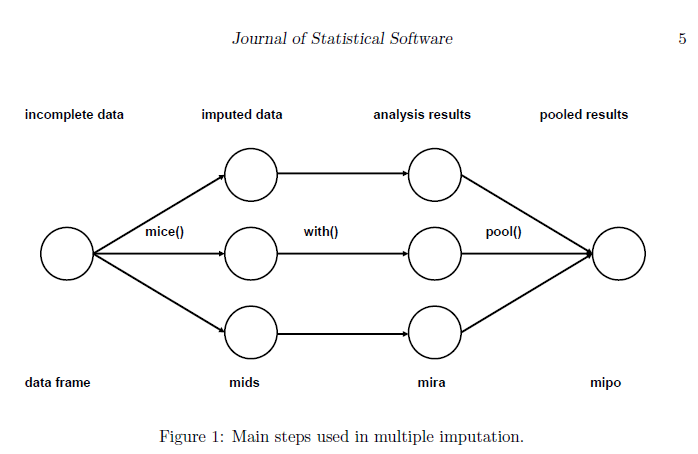
\includegraphics{images/Steps_MI.png}
\end{enumerate}

\hypertarget{selecting-the-number-of-imputations-m}{%
\paragraph{\texorpdfstring{3.1. Selecting the number of imputations
(\emph{m})}{3.1. Selecting the number of imputations (m)}}\label{selecting-the-number-of-imputations-m}}

Generally the more the better, but then the analysis takes longer to run
and it consume more computational resources. A thumb up rule regarding
the percentage of missingness is commonly used: if there is a 10\% of
missing, include 10 imputations; if there is a 20\% missing, run 20
imputations, etc.

\begin{quote}
NOTE: Although our data have more than 50\% of missing values, we will
use the default (m=5) in this example to save computation time.
\end{quote}

\hypertarget{choosing-imputation-methods.}{%
\paragraph{3.2. Choosing imputation
methods.}\label{choosing-imputation-methods.}}

There are nine methods available for imputing a variable:
\textbf{regress, pmm, truncreg, intreg, logit, ologit, mlogit, poisson
and nbreg}.

\begin{longtable}[]{@{}
  >{\centering\arraybackslash}p{(\columnwidth - 6\tabcolsep) * \real{0.2466}}
  >{\centering\arraybackslash}p{(\columnwidth - 6\tabcolsep) * \real{0.2603}}
  >{\centering\arraybackslash}p{(\columnwidth - 6\tabcolsep) * \real{0.2466}}
  >{\centering\arraybackslash}p{(\columnwidth - 6\tabcolsep) * \real{0.2466}}@{}}
\toprule\noalign{}
\begin{minipage}[b]{\linewidth}\centering
Method
\end{minipage} & \begin{minipage}[b]{\linewidth}\centering
Description
\end{minipage} & \begin{minipage}[b]{\linewidth}\centering
Scale type
\end{minipage} & \begin{minipage}[b]{\linewidth}\centering
Default
\end{minipage} \\
\midrule\noalign{}
\endhead
\bottomrule\noalign{}
\endlastfoot
pmm & Predictive mean matching & numeric & Y \\
norm & Bayesian linear regression & numeric & \\
norm.nob & Linear regression, non-Bayesian & numeric & \\
mean & Unconditional mean imputation & numeric & \\
2L.norm & Two-level linear model & numeric & \\
logreg & Logistic regression & factor, 2 levels & Y \\
polyreg & Multinomial logit model & factor, \textgreater2 levels & Y \\
polr & Ordered logit model & ordered, \textgreater2 levels & Y \\
lda & Linear discriminant analysis & factor & \\
sample & Random sample from the observed data & any & \\
\end{longtable}

\begin{itemize}
\tightlist
\item
  Which variables we want to impute? EQ5D0, bmi, ethnic, imdscore and
  smoking
\end{itemize}

The \texttt{mice} package assumes a distribution for each variable and
imputes missing variables according to that distribution. Hence, it is
important to correctly specify each of these distributions.
\texttt{mice} automatically chooses distributions for variables.

If we would like to change the methods used to impute the missing
values, we can do it by changing the methods' characteristics.

\emph{You can follow the following three lines of the code}\\
3.1 Choose the variables we want to impute\\
3.2 Save the name of the variables that will be included in the
imputation model\\
3.3 Check the imputation method used for each variable

\begin{Shaded}
\begin{Highlighting}[]
\FunctionTok{library}\NormalTok{(mice) }

\DocumentationTok{\#\#3.1) Choose the variables we want to include in the imputation model }
\FunctionTok{names}\NormalTok{(data)}

\DocumentationTok{\#\#3.2) Select them}
\NormalTok{impmodel\_var}\OtherTok{=}\FunctionTok{c}\NormalTok{(}\StringTok{"age"}\NormalTok{,}\StringTok{"sex"}\NormalTok{,}\StringTok{"ohs0"}\NormalTok{,}\StringTok{"ohsdiff"}\NormalTok{,}\StringTok{"ethnic"}\NormalTok{,}\StringTok{"eq5d0"}\NormalTok{,}\StringTok{"bmi"}\NormalTok{,}\StringTok{"imdscore"}\NormalTok{,}\StringTok{"smoking"}\NormalTok{) }\CommentTok{\#3.2}

\CommentTok{\#We run the mice code with 0 iterations (it is just for the purpose of this example)}
\NormalTok{imp }\OtherTok{\textless{}{-}} \FunctionTok{mice}\NormalTok{(data[impmodel\_var], }\AttributeTok{m=}\DecValTok{5}\NormalTok{, }\AttributeTok{maxit=}\DecValTok{0}\NormalTok{, }\AttributeTok{seed=}\DecValTok{60109}\NormalTok{)}
\CommentTok{\#Check the method mice used to impute}
\NormalTok{imp}\SpecialCharTok{$}\NormalTok{method}

\CommentTok{\#mice has identified the correct distribution for each variable. But, if you want to change the method used, you can do the following:}

\NormalTok{meth }\OtherTok{\textless{}{-}}\NormalTok{ imp}\SpecialCharTok{$}\NormalTok{method}

\CommentTok{\# Numeric variables {-} normal distribution (we are using "Linear regression, non{-}Bayesian" method to impute bmi)}
\NormalTok{norm }\OtherTok{\textless{}{-}} \FunctionTok{c}\NormalTok{(}\StringTok{"bmi"}\NormalTok{)}
\CommentTok{\# Numeric variables {-} non{-}normal distribution}
\NormalTok{nonnorm }\OtherTok{\textless{}{-}} \FunctionTok{c}\NormalTok{(}\StringTok{"eq5d0"}\NormalTok{, }\StringTok{"imdscore"}\NormalTok{)}
\CommentTok{\# Dichotomous variable}
\NormalTok{log }\OtherTok{\textless{}{-}} \FunctionTok{c}\NormalTok{(}\StringTok{"ethnic"}\NormalTok{, }\StringTok{"smoking"}\NormalTok{)}

\CommentTok{\# Turn their methods matrix into the specified imputation models}
\NormalTok{meth[norm] }\OtherTok{\textless{}{-}} \StringTok{"norm.nob"}
\NormalTok{meth[nonnorm] }\OtherTok{\textless{}{-}} \StringTok{"pmm"}
\NormalTok{meth[log] }\OtherTok{\textless{}{-}} \StringTok{"logreg"}

\NormalTok{imp2 }\OtherTok{\textless{}{-}} \FunctionTok{mice}\NormalTok{(data[impmodel\_var], }\AttributeTok{m=}\DecValTok{5}\NormalTok{, }\AttributeTok{maxit =} \DecValTok{0}\NormalTok{, }\AttributeTok{method =}\NormalTok{ meth, }\AttributeTok{seed=}\DecValTok{60109}\NormalTok{)}

\CommentTok{\#3.3) Check that mice is using the specific method}
\NormalTok{imp2}\SpecialCharTok{$}\NormalTok{method}
\end{Highlighting}
\end{Shaded}

\begin{center}\rule{0.5\linewidth}{0.5pt}\end{center}

\hypertarget{pooling-results}{%
\subsubsection{4. Pooling results}\label{pooling-results}}

The pool() function combines the estimates from m repeated complete data
analyses using Rubin's rules. The typical sequence of steps to do a
multiple imputation analysis is:

4.1. Impute the missing data by the mice function, resulting in a
multiple imputed data set (class mids);

4.2 Fit the model of interest (scientific model) on each imputed data
set by the with() function, resulting an object of class mira;\\
\emph{Classic statistical analysis has been implemented/are compatible
to with() function and can be called in the argument `expr=' (for
expression), such as linear regression} (\emph{lm()).}

4.3 Pool the estimates from each model into a single set of estimates
and standard errors, resulting is an object of class mipo;

Optionally, compare pooled estimates from different scientific models by
the pool.compare() function.

We create the impute data sets with the function \texttt{mice}:

\begin{Shaded}
\begin{Highlighting}[]
\NormalTok{impmodel\_var}\OtherTok{=}\FunctionTok{c}\NormalTok{(}\StringTok{"age"}\NormalTok{,}\StringTok{"sex"}\NormalTok{,}\StringTok{"ohs0"}\NormalTok{,}\StringTok{"ohsdiff"}\NormalTok{,}\StringTok{"ethnic"}\NormalTok{,}\StringTok{"eq5d0"}\NormalTok{,}\StringTok{"bmi"}\NormalTok{,}\StringTok{"imdscore"}\NormalTok{,}\StringTok{"smoking"}\NormalTok{)}
\NormalTok{imp }\OtherTok{=} \FunctionTok{mice}\NormalTok{(data[impmodel\_var], }\AttributeTok{maxit=}\DecValTok{10}\NormalTok{, }\AttributeTok{m =} \DecValTok{5}\NormalTok{, }\AttributeTok{seed=}\DecValTok{60109}\NormalTok{)  }\CommentTok{\#4.1}
\end{Highlighting}
\end{Shaded}

\begin{Shaded}
\begin{Highlighting}[]
\NormalTok{fit }\OtherTok{=} \FunctionTok{with}\NormalTok{(}\AttributeTok{data=}\NormalTok{imp,}\AttributeTok{expr =} \FunctionTok{lm}\NormalTok{(ohsdiff}\SpecialCharTok{\textasciitilde{}}\NormalTok{age}\SpecialCharTok{+}\NormalTok{sex}\SpecialCharTok{+}\NormalTok{bmi}\SpecialCharTok{+}\NormalTok{eq5d0}\SpecialCharTok{+}\NormalTok{ethnic}\SpecialCharTok{+}\NormalTok{imdscore}\SpecialCharTok{+}\NormalTok{smoking}\SpecialCharTok{+}\NormalTok{ohs0)) }\CommentTok{\#4.2}
\FunctionTok{summary}\NormalTok{(}\FunctionTok{pool}\NormalTok{(fit), }\AttributeTok{conf.int =} \ConstantTok{TRUE}\NormalTok{) }\CommentTok{\#4.3}
\end{Highlighting}
\end{Shaded}

\ul{\textbf{AVOID}\emph{:}}

\begin{itemize}
\item
  \emph{Averaging the data}: You might be tempted to average the
  multiply imputed data, and analyze the averaged data as if it were
  complete. This method yields incorrect standard errors, confidence
  intervals and p-values, and thus should not be used if any form of
  statistical testing or uncertainty analysis is to be done on the
  imputed data. The reason is that the procedure ignores the
  between-imputation variability, and hence shares all the drawbacks of
  single imputation
\item
  \emph{Stack imputed data}: creating m×n complete records by stacking
  the imputed data, where each record is weighted by a factor 1/m, so
  that the total sample size is equal to n.~While the estimated
  regression coefficients are unbiased, we cannot trust the standard
  errors, t-values and so on. An advantage of stacking over averaging is
  that it is easier to analyze categorical data. Although stacking can
  be useful in specific contexts, like variable selection, in general it
  is not recommended.
\end{itemize}

\begin{center}\rule{0.5\linewidth}{0.5pt}\end{center}

\hypertarget{checking-after-imputation}{%
\subsubsection{5. Checking after
imputation}\label{checking-after-imputation}}

\hypertarget{we-can-observe-which-values-has-been-imputed}{%
\paragraph{5.0 We can observe which values has been
imputed:}\label{we-can-observe-which-values-has-been-imputed}}

\begin{itemize}
\tightlist
\item
  The \texttt{stripplot()} is useful to study the distributions in data
  sets with a low number of data points.
\item
  For large data sets it is more appropriate to use the function
  \texttt{bwplot()} that produces side-by-side box-and-whisker plots for
  the observed and synthetic data.
\end{itemize}

\begin{Shaded}
\begin{Highlighting}[]
\NormalTok{impmodel\_var}\OtherTok{=}\FunctionTok{c}\NormalTok{(}\StringTok{"age"}\NormalTok{,}\StringTok{"sex"}\NormalTok{,}\StringTok{"ohs0"}\NormalTok{,}\StringTok{"ohsdiff"}\NormalTok{,}\StringTok{"ethnic"}\NormalTok{,}\StringTok{"eq5d0"}\NormalTok{,}\StringTok{"bmi"}\NormalTok{,}\StringTok{"imdscore"}\NormalTok{,}\StringTok{"smoking"}\NormalTok{) }\CommentTok{\#3.2}

\NormalTok{imp }\OtherTok{=} \FunctionTok{mice}\NormalTok{(data[impmodel\_var], }\AttributeTok{maxit=}\DecValTok{10}\NormalTok{, }\AttributeTok{m =} \DecValTok{5}\NormalTok{, }\AttributeTok{seed=}\DecValTok{60109}\NormalTok{)  }\CommentTok{\#4.1}
\end{Highlighting}
\end{Shaded}

\begin{Shaded}
\begin{Highlighting}[]
\NormalTok{fit }\OtherTok{=} \FunctionTok{with}\NormalTok{(}\AttributeTok{data=}\NormalTok{imp,}\AttributeTok{expr =} \FunctionTok{lm}\NormalTok{(ohsdiff}\SpecialCharTok{\textasciitilde{}}\NormalTok{age}\SpecialCharTok{+}\NormalTok{sex}\SpecialCharTok{+}\NormalTok{bmi}\SpecialCharTok{+}\NormalTok{eq5d0}\SpecialCharTok{+}\NormalTok{ethnic}\SpecialCharTok{+}\NormalTok{imdscore}\SpecialCharTok{+}\NormalTok{smoking}\SpecialCharTok{+}\NormalTok{ohs0)) }\CommentTok{\#4.2}
\FunctionTok{summary}\NormalTok{(}\FunctionTok{pool}\NormalTok{(fit), }\AttributeTok{conf.int =} \ConstantTok{TRUE}\NormalTok{) }\CommentTok{\#4.3}

\CommentTok{\#Observe which values has been imputed}
\FunctionTok{stripplot}\NormalTok{(imp) }\CommentTok{\#blue = observed data; red = imputed data}
\end{Highlighting}
\end{Shaded}

\begin{Shaded}
\begin{Highlighting}[]
\FunctionTok{bwplot}\NormalTok{(imp)    }\CommentTok{\#blue = observed data; red = imputed data}
\end{Highlighting}
\end{Shaded}

\hypertarget{evaluate-differences-between-observed-and-imputed-data}{%
\paragraph{5.1 Evaluate differences between observed and imputed
data:}\label{evaluate-differences-between-observed-and-imputed-data}}

\hypertarget{observe-their-distribution-before-observed-and-after-imputed-data}{%
\subparagraph{5.1.1. Observe their distribution before (observed) and
after (imputed
data):}\label{observe-their-distribution-before-observed-and-after-imputed-data}}

\begin{Shaded}
\begin{Highlighting}[]
\FunctionTok{densityplot}\NormalTok{(imp) }\CommentTok{\#blue line = observed data; red lines = imputed data }
\end{Highlighting}
\end{Shaded}

\textbf{Quiz}

\begin{itemize}
\tightlist
\item
  Do you think distributions match up well?
\end{itemize}

\hypertarget{compare-the-distributions-of-observed-and-imputed-data-conditional-on-the-missingness-probability.}{%
\subparagraph{5.1.2. Compare the distributions of observed and imputed
data conditional on the missingness
probability.}\label{compare-the-distributions-of-observed-and-imputed-data-conditional-on-the-missingness-probability.}}

Interpretation is more difficult if discrepancies are shown in the
density plot. Such discrepancies may be caused by a bad imputation
model, by a missing data mechanism that is not MCAR or by a combination
of both.

If there are discrepancies, Bondarenko and Raghunathan (2016) proposed a
more refined diagnostic tool that aims to compare the distributions of
observed and imputed data conditional on the missingness probability.
The idea is that \ul{under MAR the conditional distributions should be
similar if the assumed model for creating multiple imputations has a
good fit}. An example is created as:

\begin{Shaded}
\begin{Highlighting}[]
\CommentTok{\#Model the probability of each record being incomplete as a function of all variables in each imputed data set.}
\NormalTok{fit }\OtherTok{\textless{}{-}} \FunctionTok{with}\NormalTok{(imp, }\FunctionTok{glm}\NormalTok{(}\FunctionTok{ici}\NormalTok{(imp)}\SpecialCharTok{\textasciitilde{}}\NormalTok{ohsdiff}\SpecialCharTok{+}\NormalTok{age}\SpecialCharTok{+}\NormalTok{sex}\SpecialCharTok{+}\NormalTok{bmi}\SpecialCharTok{+}\NormalTok{eq5d0}\SpecialCharTok{+}\NormalTok{ethnic}\SpecialCharTok{+}\NormalTok{imdscore}\SpecialCharTok{+}\NormalTok{smoking}\SpecialCharTok{+}\NormalTok{ohs0, }\AttributeTok{family =}\NormalTok{ binomial)) }

\CommentTok{\# The probabilities (propensities) are then averaged over the imputed datasets to obtain stability.}
\NormalTok{ps }\OtherTok{\textless{}{-}} \FunctionTok{rep}\NormalTok{(}\FunctionTok{rowMeans}\NormalTok{(}\FunctionTok{sapply}\NormalTok{(fit}\SpecialCharTok{$}\NormalTok{analyses, fitted.values)),}
\NormalTok{          imp}\SpecialCharTok{$}\NormalTok{m }\SpecialCharTok{+} \DecValTok{1}\NormalTok{)}

\CommentTok{\#Plot the each variable against the propensity score in each dataset:}
\CommentTok{\#blue = observed data; red = imputed data}
\FunctionTok{xyplot}\NormalTok{(imp, bmi }\SpecialCharTok{\textasciitilde{}}\NormalTok{ ps }\SpecialCharTok{|} \FunctionTok{as.factor}\NormalTok{(.imp),}
       \AttributeTok{xlab =} \StringTok{"Probability that record is incomplete"}\NormalTok{,}
       \AttributeTok{ylab =} \StringTok{"BMI"}\NormalTok{, }\AttributeTok{pch =} \FunctionTok{c}\NormalTok{(}\DecValTok{1}\NormalTok{, }\DecValTok{19}\NormalTok{), }\AttributeTok{col =} \FunctionTok{mdc}\NormalTok{(}\DecValTok{1}\SpecialCharTok{:}\DecValTok{2}\NormalTok{))}
\end{Highlighting}
\end{Shaded}

\begin{Shaded}
\begin{Highlighting}[]
\FunctionTok{xyplot}\NormalTok{(imp, eq5d0 }\SpecialCharTok{\textasciitilde{}}\NormalTok{ ps }\SpecialCharTok{|} \FunctionTok{as.factor}\NormalTok{(.imp),}
       \AttributeTok{xlab =} \StringTok{"Probability that record is incomplete"}\NormalTok{,}
       \AttributeTok{ylab =} \StringTok{"EQ5D0"}\NormalTok{, }\AttributeTok{pch =} \FunctionTok{c}\NormalTok{(}\DecValTok{1}\NormalTok{, }\DecValTok{19}\NormalTok{), }\AttributeTok{col =} \FunctionTok{mdc}\NormalTok{(}\DecValTok{1}\SpecialCharTok{:}\DecValTok{2}\NormalTok{))}
\end{Highlighting}
\end{Shaded}

\begin{Shaded}
\begin{Highlighting}[]
\FunctionTok{xyplot}\NormalTok{(imp, ethnic }\SpecialCharTok{\textasciitilde{}}\NormalTok{ ps }\SpecialCharTok{|} \FunctionTok{as.factor}\NormalTok{(.imp),}
       \AttributeTok{xlab =} \StringTok{"Probability that record is incomplete"}\NormalTok{,}
       \AttributeTok{ylab =} \StringTok{"Ethnic"}\NormalTok{, }\AttributeTok{pch =} \FunctionTok{c}\NormalTok{(}\DecValTok{1}\NormalTok{, }\DecValTok{19}\NormalTok{), }\AttributeTok{col =} \FunctionTok{mdc}\NormalTok{(}\DecValTok{1}\SpecialCharTok{:}\DecValTok{2}\NormalTok{))}
\end{Highlighting}
\end{Shaded}

\begin{Shaded}
\begin{Highlighting}[]
\FunctionTok{xyplot}\NormalTok{(imp, imdscore }\SpecialCharTok{\textasciitilde{}}\NormalTok{ ps }\SpecialCharTok{|} \FunctionTok{as.factor}\NormalTok{(.imp),}
       \AttributeTok{xlab =} \StringTok{"Probability that record is incomplete"}\NormalTok{,}
       \AttributeTok{ylab =} \StringTok{"imdscore"}\NormalTok{, }\AttributeTok{pch =} \FunctionTok{c}\NormalTok{(}\DecValTok{1}\NormalTok{, }\DecValTok{19}\NormalTok{), }\AttributeTok{col =} \FunctionTok{mdc}\NormalTok{(}\DecValTok{1}\SpecialCharTok{:}\DecValTok{2}\NormalTok{))}
\end{Highlighting}
\end{Shaded}

\begin{Shaded}
\begin{Highlighting}[]
\FunctionTok{xyplot}\NormalTok{(imp, smoking }\SpecialCharTok{\textasciitilde{}}\NormalTok{ ps }\SpecialCharTok{|} \FunctionTok{as.factor}\NormalTok{(.imp),}
       \AttributeTok{xlab =} \StringTok{"Probability that record is incomplete"}\NormalTok{,}
       \AttributeTok{ylab =} \StringTok{"Smoking"}\NormalTok{, }\AttributeTok{pch =} \FunctionTok{c}\NormalTok{(}\DecValTok{1}\NormalTok{, }\DecValTok{19}\NormalTok{), }\AttributeTok{col =} \FunctionTok{mdc}\NormalTok{(}\DecValTok{1}\SpecialCharTok{:}\DecValTok{2}\NormalTok{))}
\end{Highlighting}
\end{Shaded}

In this case, the distributions of the blue and red points are quite
similar, as expected under MAR.

\hypertarget{compare-complete-results-vs-imputed-results}{%
\subparagraph{5.1.3. Compare complete results vs imputed
results}\label{compare-complete-results-vs-imputed-results}}

Observe the differences in the estimates and confidence intervals:

\begin{Shaded}
\begin{Highlighting}[]
\CommentTok{\#Complete cases results:variables names, OR, Low and High CI}
\NormalTok{fit0 }\OtherTok{=}\FunctionTok{lm}\NormalTok{(ohsdiff}\SpecialCharTok{\textasciitilde{}}\NormalTok{age}\SpecialCharTok{+}\NormalTok{sex}\SpecialCharTok{+}\NormalTok{bmi}\SpecialCharTok{+}\NormalTok{eq5d0}\SpecialCharTok{+}\NormalTok{ethnic}\SpecialCharTok{+}\NormalTok{imdscore}\SpecialCharTok{+}\NormalTok{smoking}\SpecialCharTok{+}\NormalTok{ohs0, }\AttributeTok{data=}\FunctionTok{na.omit}\NormalTok{(data))}
\FunctionTok{print}\NormalTok{(}\StringTok{"Using complete cases"}\NormalTok{)}
\FunctionTok{print}\NormalTok{( }\FunctionTok{cbind}\NormalTok{(}\AttributeTok{OR=}\FunctionTok{summary}\NormalTok{(fit0)}\SpecialCharTok{$}\NormalTok{coefficients[,}\DecValTok{1}\NormalTok{],}\FunctionTok{confint}\NormalTok{(fit0)) )}

\CommentTok{\#Imputed results: variables names, OR, Low and High CI}
\NormalTok{fit }\OtherTok{=} \FunctionTok{with}\NormalTok{(}\AttributeTok{data=}\NormalTok{imp,}\AttributeTok{expr =} \FunctionTok{lm}\NormalTok{(ohsdiff}\SpecialCharTok{\textasciitilde{}}\NormalTok{age}\SpecialCharTok{+}\NormalTok{sex}\SpecialCharTok{+}\NormalTok{bmi}\SpecialCharTok{+}\NormalTok{eq5d0}\SpecialCharTok{+}\NormalTok{ethnic}\SpecialCharTok{+}\NormalTok{imdscore}\SpecialCharTok{+}\NormalTok{smoking}\SpecialCharTok{+}\NormalTok{ohs0))}
\FunctionTok{print}\NormalTok{(}\StringTok{"Using imputed data"}\NormalTok{)}
\FunctionTok{summary}\NormalTok{(}\FunctionTok{pool}\NormalTok{(fit), }\AttributeTok{conf.int =} \ConstantTok{TRUE}\NormalTok{)[}\FunctionTok{c}\NormalTok{(}\DecValTok{1}\NormalTok{,}\DecValTok{2}\NormalTok{,}\DecValTok{7}\NormalTok{,}\DecValTok{8}\NormalTok{)]}
\end{Highlighting}
\end{Shaded}

Interpretation: After imputation, age is significant in our model.
Results regarding all other variables seems to be consistent before and
after imputation.

\begin{center}\rule{0.5\linewidth}{0.5pt}\end{center}

\hypertarget{what-to-do-when-a-statistical-analysis-is-not-compatible-with-with-function}{%
\subsubsection{6. What to do when a statistical analysis is not
compatible with with()
function}\label{what-to-do-when-a-statistical-analysis-is-not-compatible-with-with-function}}

There might be cases where an analysis is such complex that you won't be
able to use the function with(). For this cases, the alternative is to
store the imputed data sets into a list, run the desired methods using a
loop, and later combine the results using Rubin's rules.

6.1 Run imputation\\
6.2 Extract the imputed data sets: imp.data is a data.frame that
contains all the imputed data sets, which are distinguishable by the
variable .imp\\
6.3 See de number of individuals for each imputed data set\\
6.4 Create a list for storing the results where the length is the number
if imputed data sets\\
6.5 Run a loop for each of the imputed data sets and store the results
in the list created in the previous step.\\
6.6 Transform the list into a mira object to perform the pooling\\
6.7 Pool the results

\begin{Shaded}
\begin{Highlighting}[]
\NormalTok{impmodel\_var}\OtherTok{=}\FunctionTok{c}\NormalTok{(}\StringTok{"age"}\NormalTok{,}\StringTok{"sex"}\NormalTok{,}\StringTok{"ohs0"}\NormalTok{,}\StringTok{"ohsdiff"}\NormalTok{,}\StringTok{"ethnic"}\NormalTok{,}\StringTok{"eq5d0"}\NormalTok{,}\StringTok{"bmi"}\NormalTok{,}\StringTok{"imdscore"}\NormalTok{,}\StringTok{"smoking"}\NormalTok{)}\CommentTok{\#3.2}

\NormalTok{imp }\OtherTok{=} \FunctionTok{mice}\NormalTok{(data[impmodel\_var], }\AttributeTok{maxit=}\DecValTok{10}\NormalTok{, }\AttributeTok{m =} \DecValTok{5}\NormalTok{, }\AttributeTok{seed=}\DecValTok{60109}\NormalTok{)   }\CommentTok{\#6.1}
\NormalTok{imp.data }\OtherTok{=} \FunctionTok{complete}\NormalTok{(imp , }\StringTok{"long"}\NormalTok{)   }\CommentTok{\#6.2}
\FunctionTok{table}\NormalTok{(imp.data}\SpecialCharTok{$}\NormalTok{.imp)                }\CommentTok{\#6.3}
\NormalTok{Fit.list }\OtherTok{=} \FunctionTok{vector}\NormalTok{(}\StringTok{"list"}\NormalTok{, }\FunctionTok{length}\NormalTok{(}\FunctionTok{unique}\NormalTok{(imp.data}\SpecialCharTok{$}\NormalTok{.imp))) }\CommentTok{\#6.4}
\NormalTok{Fit.list2}\OtherTok{=} \FunctionTok{vector}\NormalTok{(}\StringTok{"list"}\NormalTok{, }\FunctionTok{length}\NormalTok{(}\FunctionTok{unique}\NormalTok{(imp.data}\SpecialCharTok{$}\NormalTok{.imp))) }\CommentTok{\#6.4}
\ControlFlowTok{for}\NormalTok{ (i }\ControlFlowTok{in} \FunctionTok{unique}\NormalTok{(imp.data}\SpecialCharTok{$}\NormalTok{.imp)) \{  }\CommentTok{\#6.5 Loop start}
\NormalTok{      fit }\OtherTok{=} \FunctionTok{lm}\NormalTok{(ohsdiff}\SpecialCharTok{\textasciitilde{}}\NormalTok{age}\SpecialCharTok{+}\NormalTok{sex}\SpecialCharTok{+}\NormalTok{ethnic}\SpecialCharTok{+}\NormalTok{eq5d0}\SpecialCharTok{+}\NormalTok{imdscore}\SpecialCharTok{+}\NormalTok{bmi}\SpecialCharTok{+}\NormalTok{smoking}\SpecialCharTok{+}\NormalTok{ohs0, }\AttributeTok{data =}\NormalTok{ imp.data[imp.data}\SpecialCharTok{$}\NormalTok{.imp }\SpecialCharTok{==}\NormalTok{ i,])}
\NormalTok{      Fit.list[[i]]}\OtherTok{=} \FunctionTok{summary}\NormalTok{(fit)}
\NormalTok{                                  \} }\CommentTok{\#6.5 Loop end}
\NormalTok{Fit.list.mira }\OtherTok{=} \FunctionTok{as.mira}\NormalTok{(Fit.list)   }\CommentTok{\#6.6 }
\end{Highlighting}
\end{Shaded}

\begin{Shaded}
\begin{Highlighting}[]
\FunctionTok{summary}\NormalTok{(}\FunctionTok{pool}\NormalTok{(Fit.list.mira),}\AttributeTok{conf.int =} \ConstantTok{TRUE}\NormalTok{) }\CommentTok{\#6.7}
\end{Highlighting}
\end{Shaded}


\end{document}
